\thispagestyle{fancy}

\section{Untersuchung optisch gepumpter Laserstrukturen auf unterschiedlichen Templates}

Dieses Kapitel widmet sich der Untersuchung zweier Probenreihen von optisch gepumpten Laserstrukturen, die aus Rezepten aus zwei unterschiedlichen Serien stammen. Die beiden Serien unterscheiden sich im wesentlichen dadurch, dass sie mit(Serie 2) und ohne Übergitter(Serie 1)gewachsen wurden. 
Die Proben weisen untereinander Unterschiede in ihren Substraten auf, so sind zwei Proben der Serie 1 auf AlN-Bulk zweier unterschiedlicher Hersteller (HexaTech, IKZ) gewachsen und alle anderen Proben auf ELO AlN/Sapphire mit jeweils 3 unterschiedlichen "Offcut"-Winkeln. Tabellarisch sieht die Zusammenstellung wie folgt aus: 

\vspace{1cm}
\setlength{\arrayrulewidth}{0.05mm}
\setlength{\tabcolsep}{2.5mm}
\renewcommand{\arraystretch}{1}
\centering
\begin{tabular}{ |c|c|c|c|c|c|   }
\hline
\multicolumn{3}{|c|}{Serie 1} & \multicolumn{3}{c|}{Serie 2}  \\
\hline
Name & offcut& Template & Name& offcut & Template \\
\hline
A & 0.1$^\circ$m & ELO & A-SL & 0.1$^\circ$m & ELO \\
B & 0.1$^\circ$m* & ELO & B-SL & 0.1$^\circ$m* & ELO \\
C & 0.2$^\circ$m & ELO & C-SL & 0.2$^\circ$m & ELO \\
D & 0.1$^\circ$m & Bulk(IKZ) &  & &  \\
E & 0.1$^\circ$m & Bulk(Hexatech) & & & \\
\hline
\end{tabular}
\vspace{1cm}
\raggedright
\newline
Die Untersuchung des Einflusses des Fehlschnitt-Winkels des Substrates, ist insofern interessant, da dieser eine entscheidende Rolle beim Wachstum der Heterostrukturen spielt. Er erlaubt es die Wachstumskinetik zu steuern, so dass sich die Schichten in die kristalline Struktur  formen wie in Abbildung \ref{fig:offcut} zu sehen ist.
Der Fehlschnitt-Winkel $\alpha$ ist die Winkel-Differenz zwischen Oberflächennormale und der c-Richtung. Für ein $\alpha \leq 0,12 $ wurde gezeigt, dass es zu Stufenfluss kommt und somit zu relativ glatten Oberflächen mit wellenartiger Morphologie und mit $\alpha \geq 0,16 $ in Stufenbündelwachstum mit Makrostufen resultieren kann. Dies ist nicht unwichtig für Laserstrukturen, da glatte Oberflächen optische Streuung an der Oberfläche verringern, sollten aber keinen Effekt auf die IQE haben. Allerdings kann an den Stufenkanten verstärkt Ga eingebaut und somit die Zusammensetzung der aktiven Zone inhomogen werden \cite{zeimeru} \cite{MOGILATENKO2014222} \cite{fmehnke}, was wiederum einen Einfluss auf die IQE durch Lokalisierung haben könnte.
%
\begin{figure}[htb]
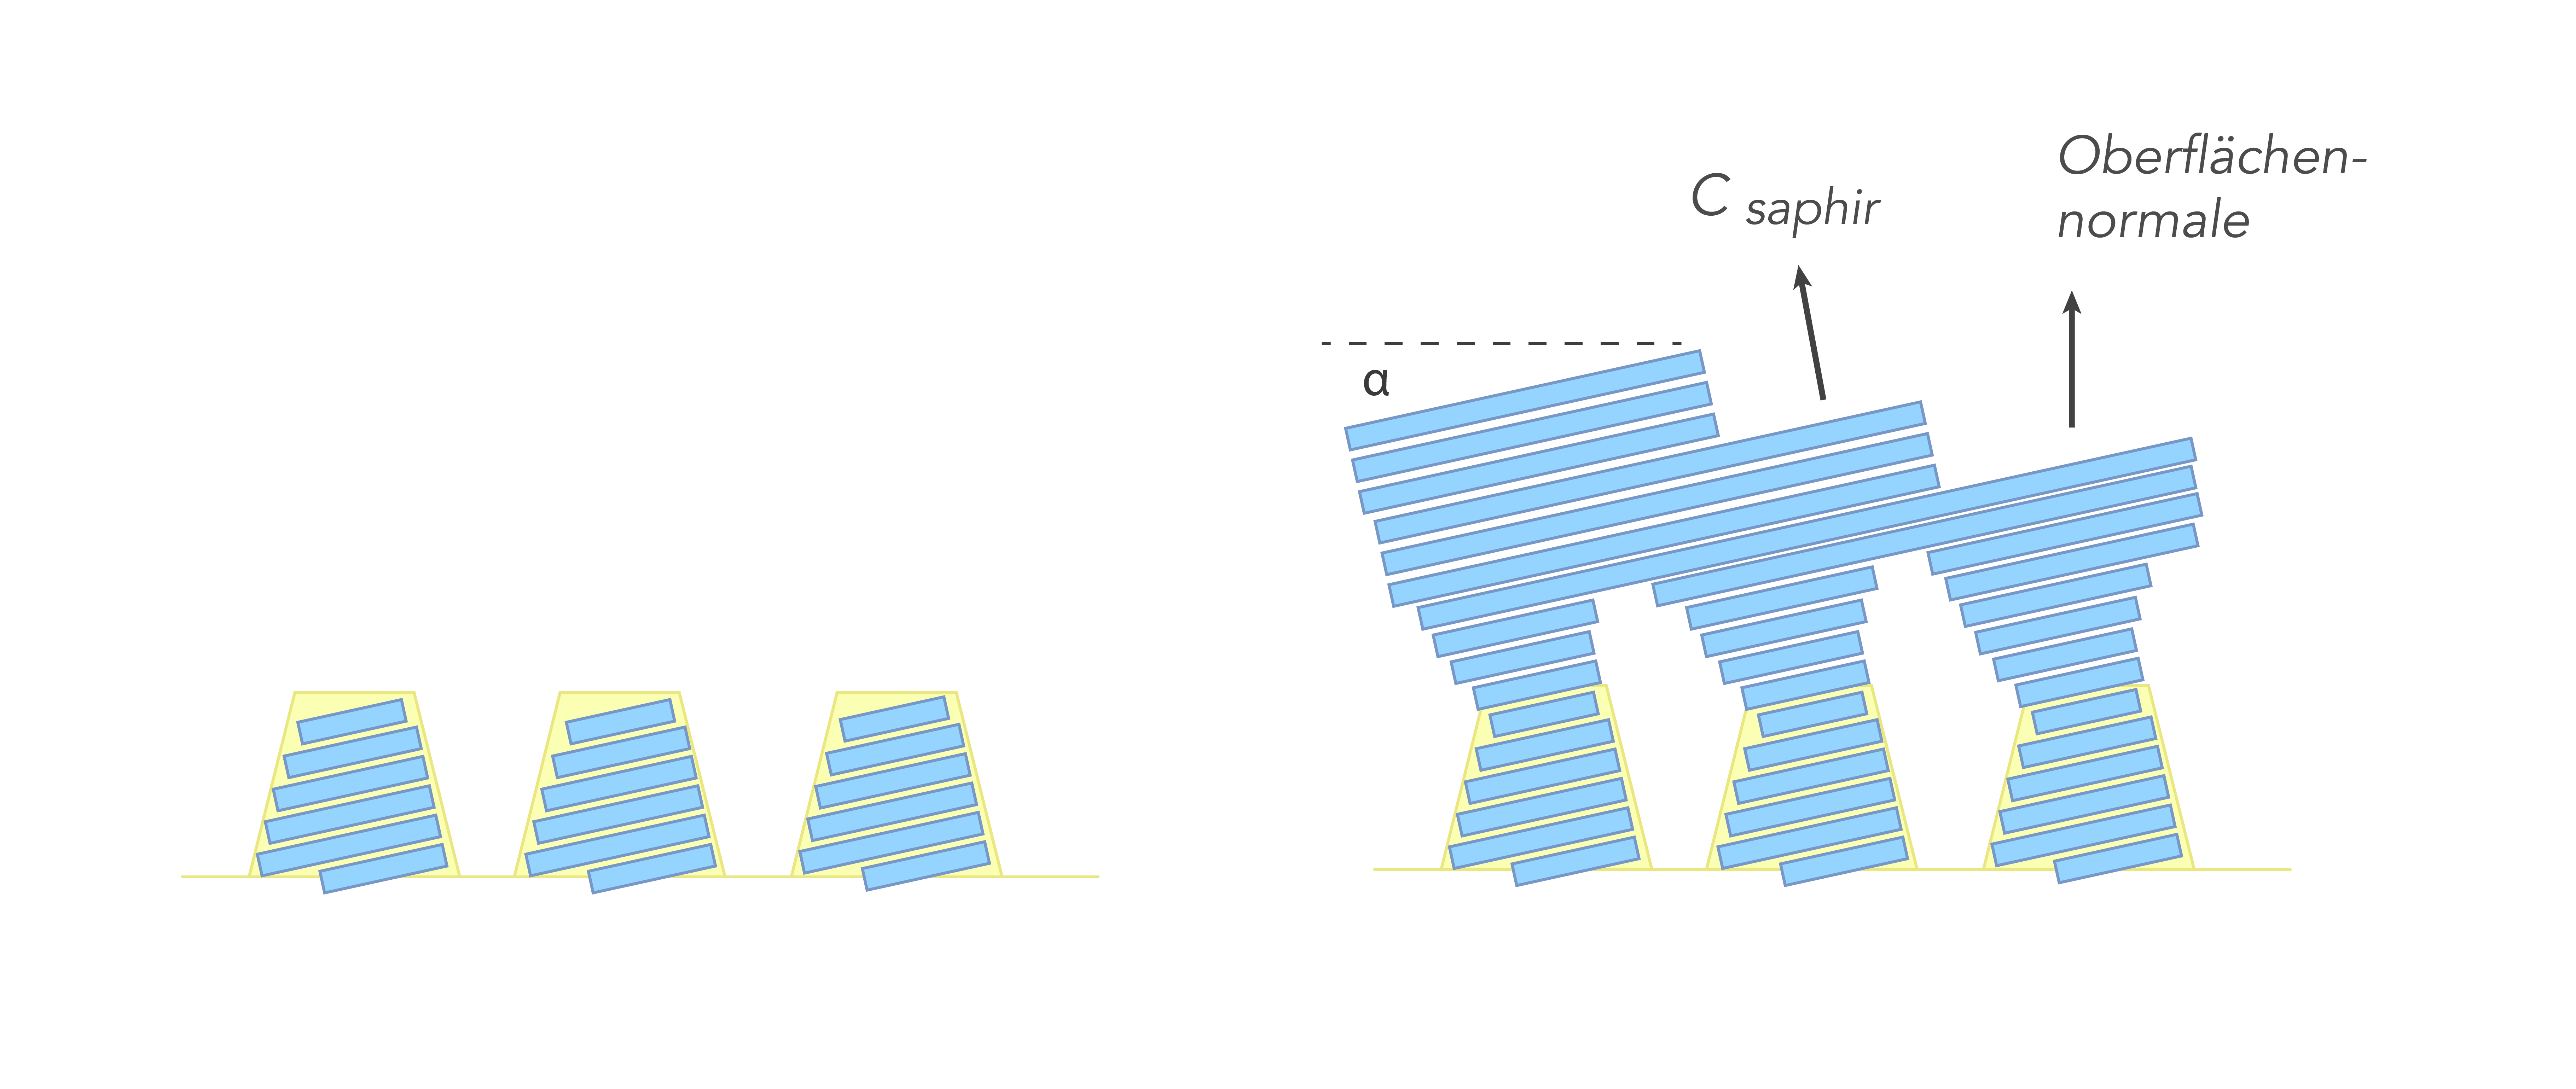
\includegraphics[width=\linewidth]{Bilder/offcut.png}
\caption{Einfluss des Fehlschnitt-Winkels auf das Wachstum bei ELO AlN/Saphir.}
\label{fig:offcut}
\end{figure}
\raggedright
\vspace{1cm}
%
Die Makrostufen können allerdings zu einer Reduktion der TDD beitragen, die wiederum in der IQE sichtbar ist \ref{fig:IQEthreadingdisl}. Bei Proben mit einem geringen Fehlschnitt von $\alpha = 0,12 $ verlaufen die Versetzungen senkrecht zur Kristalloberfläche. Bei Proben mit einem großen Fehlschnitt von $\alpha = 0,16 $ verlaufen die Versetzungen diagonal. Bei diesen Versetzungen handelt es sich um sogenannten Koaleszenzkorngrenzen die an der Oberfläche als Makrostufen zu erkennen sind \cite{MOGILATENKO2014222}. 
%
\begin{figure}[htb]
  \centering
  \begin{minipage}[t]{0.49\textwidth}
    \centering
    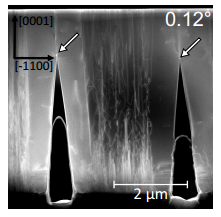
\includegraphics[width=\textwidth]{Bilder/offcutsenkrecht.png}
    \label{}
  \end{minipage}
	\hfill
  \begin{minipage}[t]{0.49\textwidth}
    \centering
    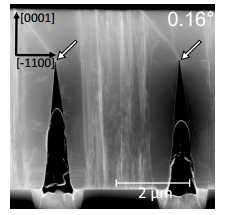
\includegraphics[width=\linewidth]{Bilder/offcutdiagonal.png}
    \label{}
  \end{minipage}
	\caption{Querschnitts-TEM-Aufnahmen mit den sichtbaren senkrecht und diagonal verlaufenden Schraubenversetzungen}
\end{figure}
%
Bei Schichtdicken $ \geq 10 \mu m $ kreuzen diese diagonal verlaufenden Makrostufen die versetzungsreichen Gebiete zwischen den geätzten Gräben im ELO oft genug um diese fast vollständig zu annhilieren \cite{fmehnke}. Bei den hier verwendeten Schichtdicken von $ \geq 1 \thinspace \mu m $ ist nur eine teilweise Annihilation und damit eine Defektreduktion von $1\cdot 10^{10} \thinspace cm^{-2}$ auf $5\cdot 10^9 \thinspace cm^{-2}$ zu erwarten \cite{fmehnke}. Weiter beachtet werden muss, dass bei den darauf folgenden Schichten eine Planarisierung stattfinden muss, um möglichst ebene aktive Zone zu haben. 


\subsection{UVC-Laser Strukturen auf ELO ohne Übergitter}
%
\begin{figure}[htb]
  \centering
  \begin{minipage}[t]{0.30\textwidth}
    \centering
    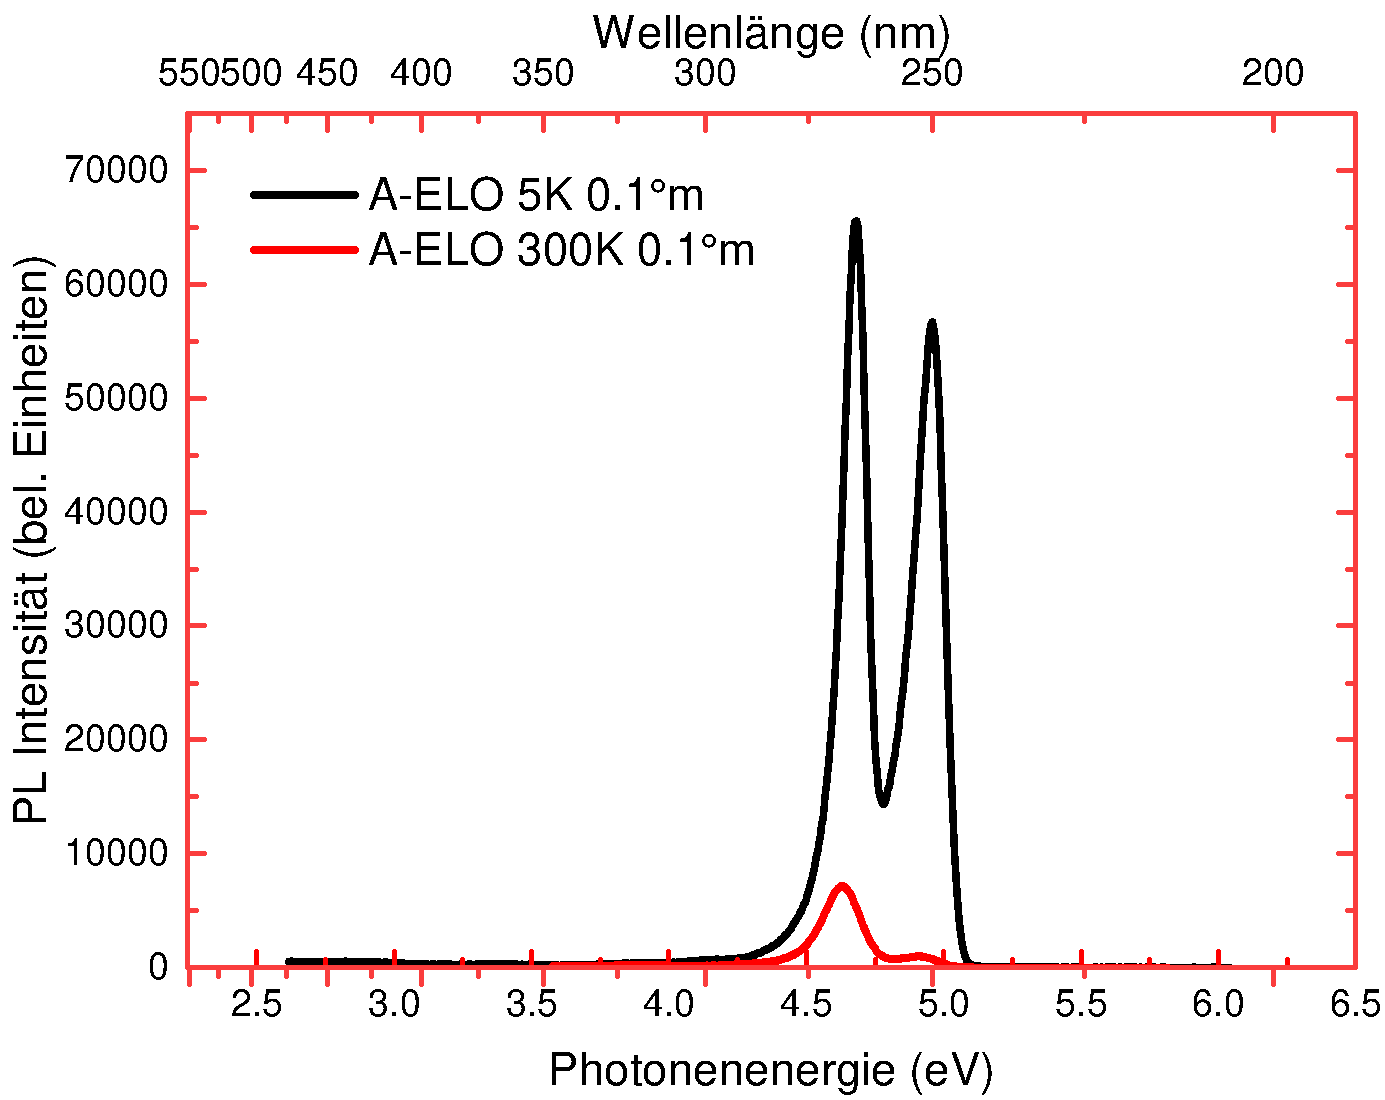
\includegraphics[width=\textwidth]{Bilder/TS4045/aelo.pdf}
  \end{minipage}
	\hfill
  \begin{minipage}[t]{0.30\textwidth}
    \centering
    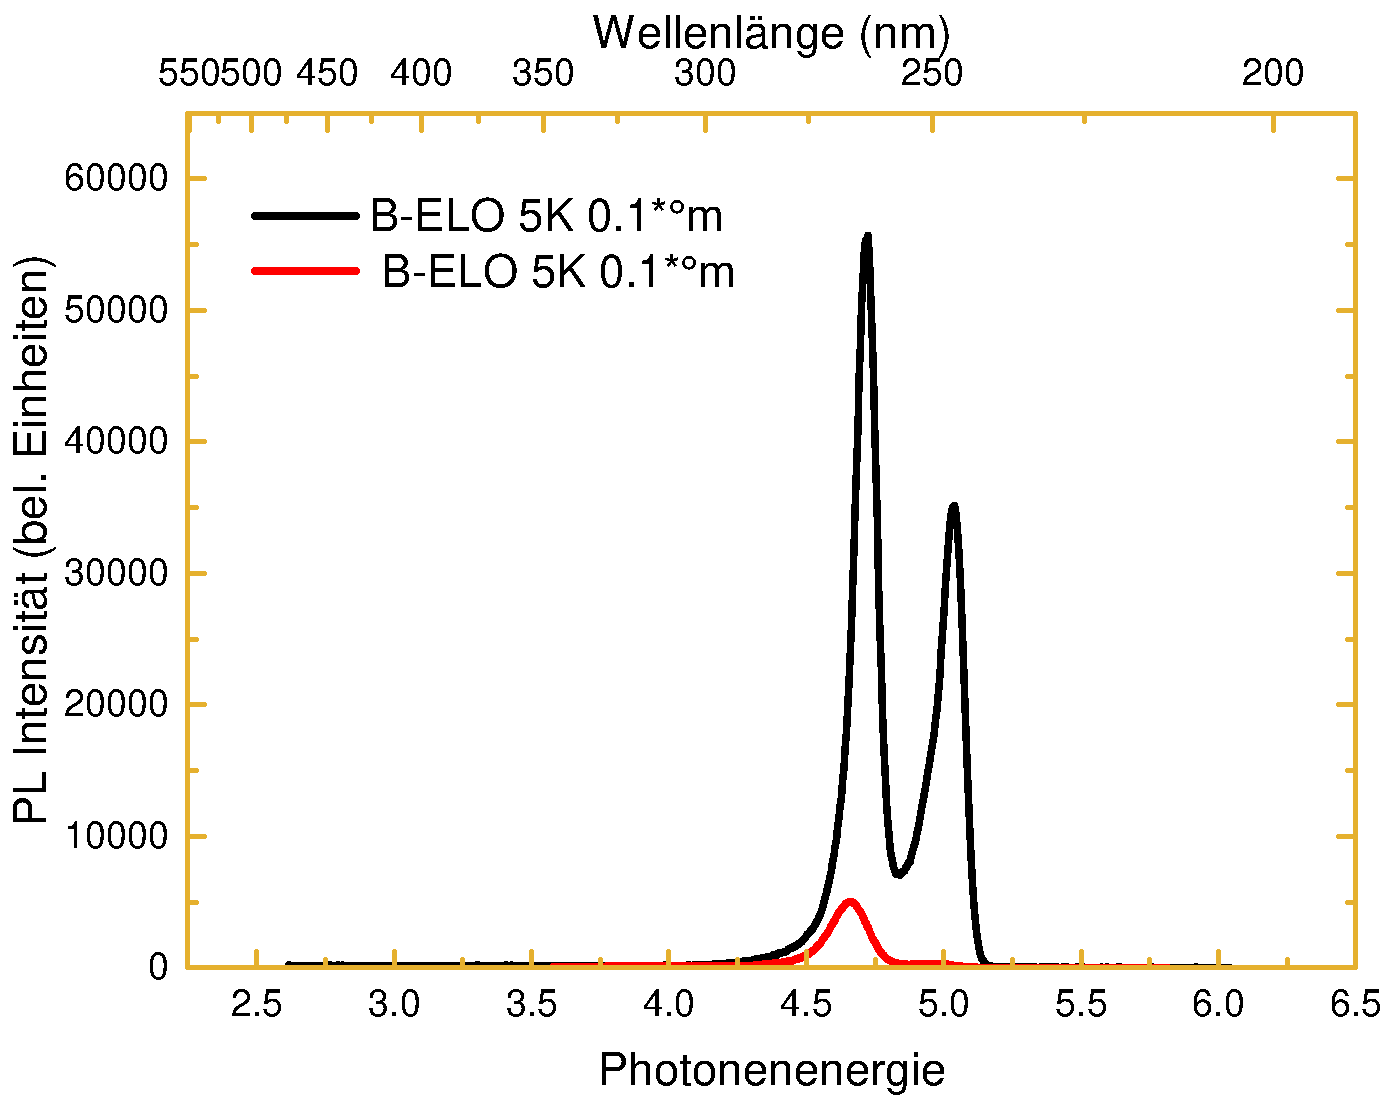
\includegraphics[width=\linewidth]{Bilder/TS4045/belo.pdf}
  \end{minipage}
	\hfill
  \begin{minipage}[t]{0.30\textwidth}
    \centering
    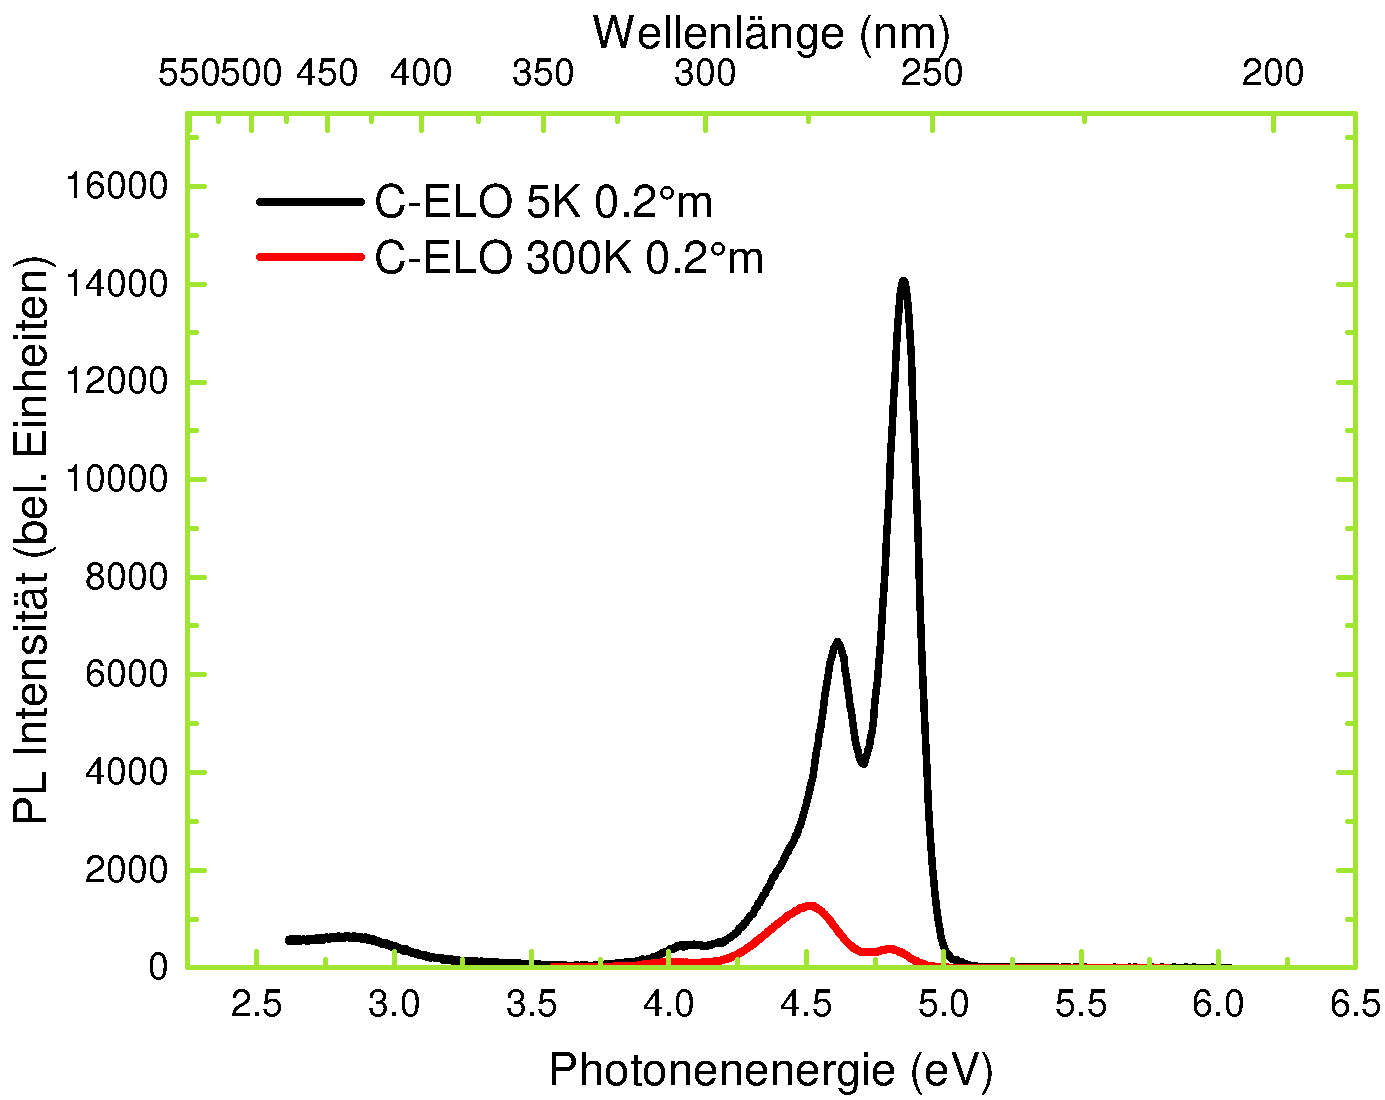
\includegraphics[width=\linewidth]{Bilder/TS4045/celo.pdf}
  \end{minipage}
	\caption{Aufnahme der Spektren der Proben A-ELO mit einem Fehlschnittwinkel von $0.1$ in die Standard m-Richtung, Probe B-ELO mit einem Fehlschnittwinkel von $0.1$ die andere m-Richtung und Probe C-ELO mit einem Fehlschnittwinkel von $0.2$ in die standard m-Richtung. }
\end{figure}
%
Die untersuchten Proben haben alle eine aktive Zone, die sich zusammen setzt aus zwei $5$nm dicken und siliziumdotierten $ Al_{0.8}Ga_{0.3}N$-Barrieren und drei $2.2$nm dicken $ Al_{0.56}Ga_{0.44}N$ QWs zusammen mit 
%
\begin{figure}[htb]
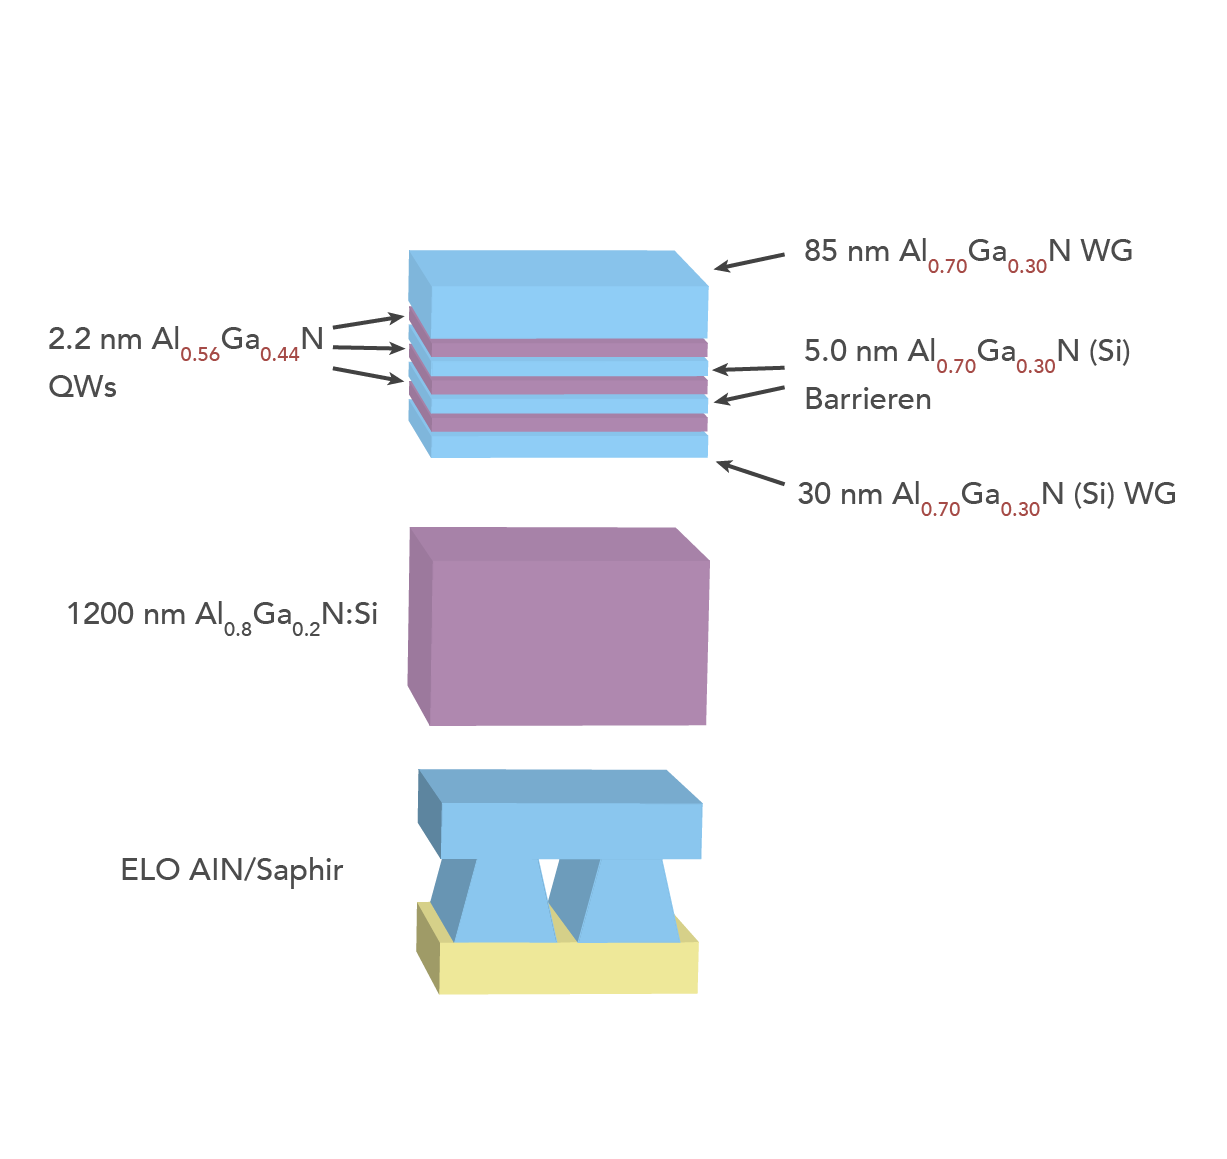
\includegraphics[width=\linewidth]{Bilder/TS4045/ts4045.png}
\caption{Schichtstruktur der untersuchten Proben.}
\label{fig:offcut}
\end{figure}
\raggedright
\vspace{1cm}
%
\begin{figure}[htb]
  \centering
  \begin{minipage}[t]{0.49\textwidth}
    \centering
    \includegraphics[width=\textwidth]{Bilder/TS4045/iqeRT.pdf}
    \label{}
  \end{minipage}
	\hfill
  \begin{minipage}[t]{0.49\textwidth}
    \centering
    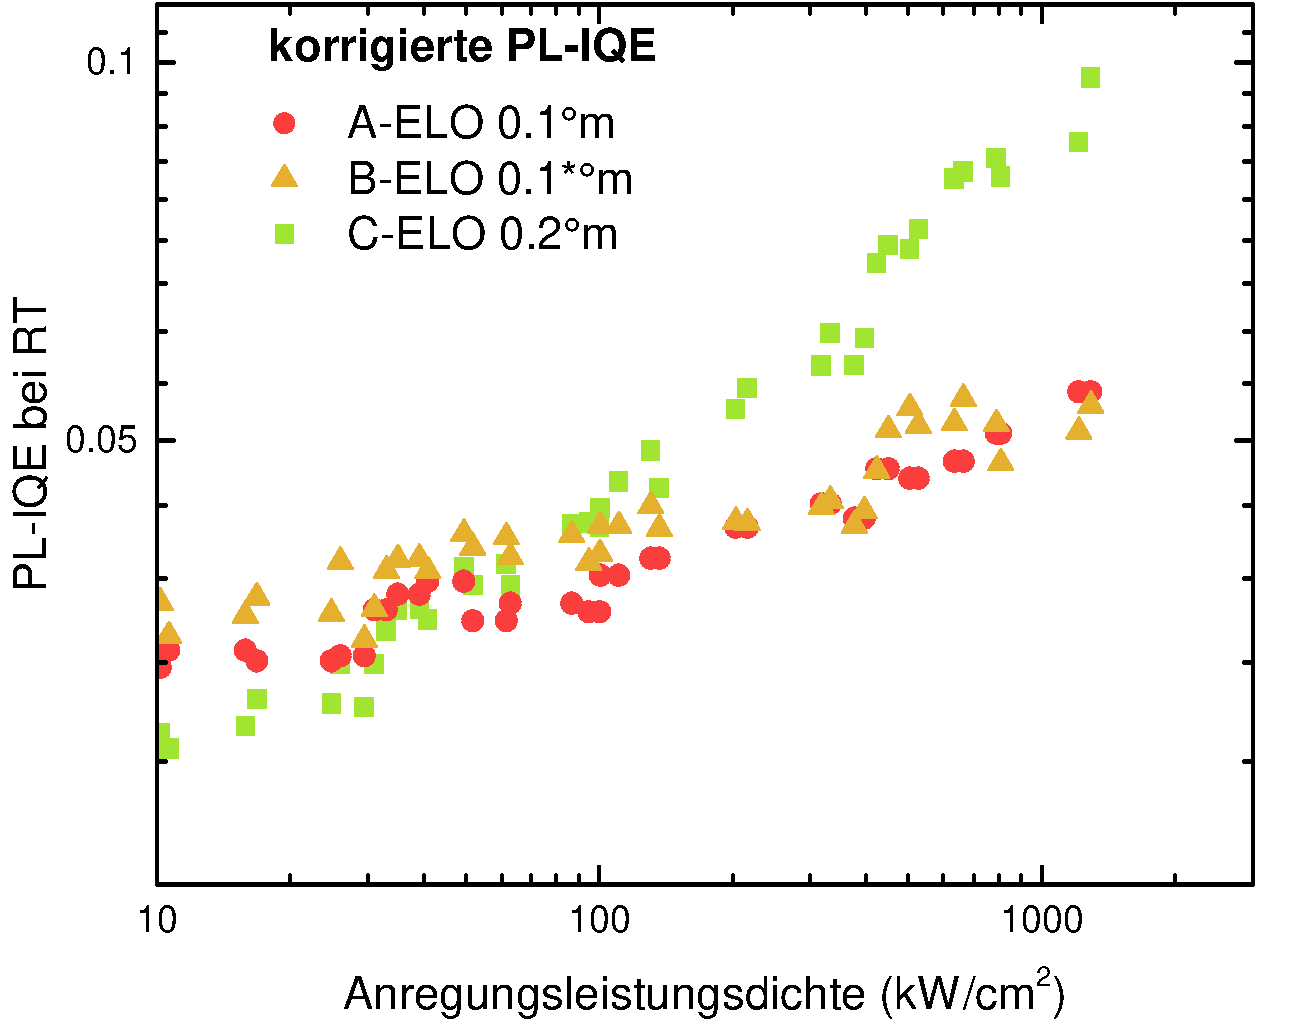
\includegraphics[width=\linewidth]{Bilder/TS4045/corrIQERT.pdf}
    \label{}
  \end{minipage}
	\caption{Die Standard-IQE und die korrigierte IQE bei Raumtemperatur. Die korrigierte IQE fällt deutlich geringer aus für alle Proben.}
\end{figure}
%
%
\begin{figure}[htb]
  \centering
  \begin{minipage}[t]{0.49\textwidth}
    \centering
    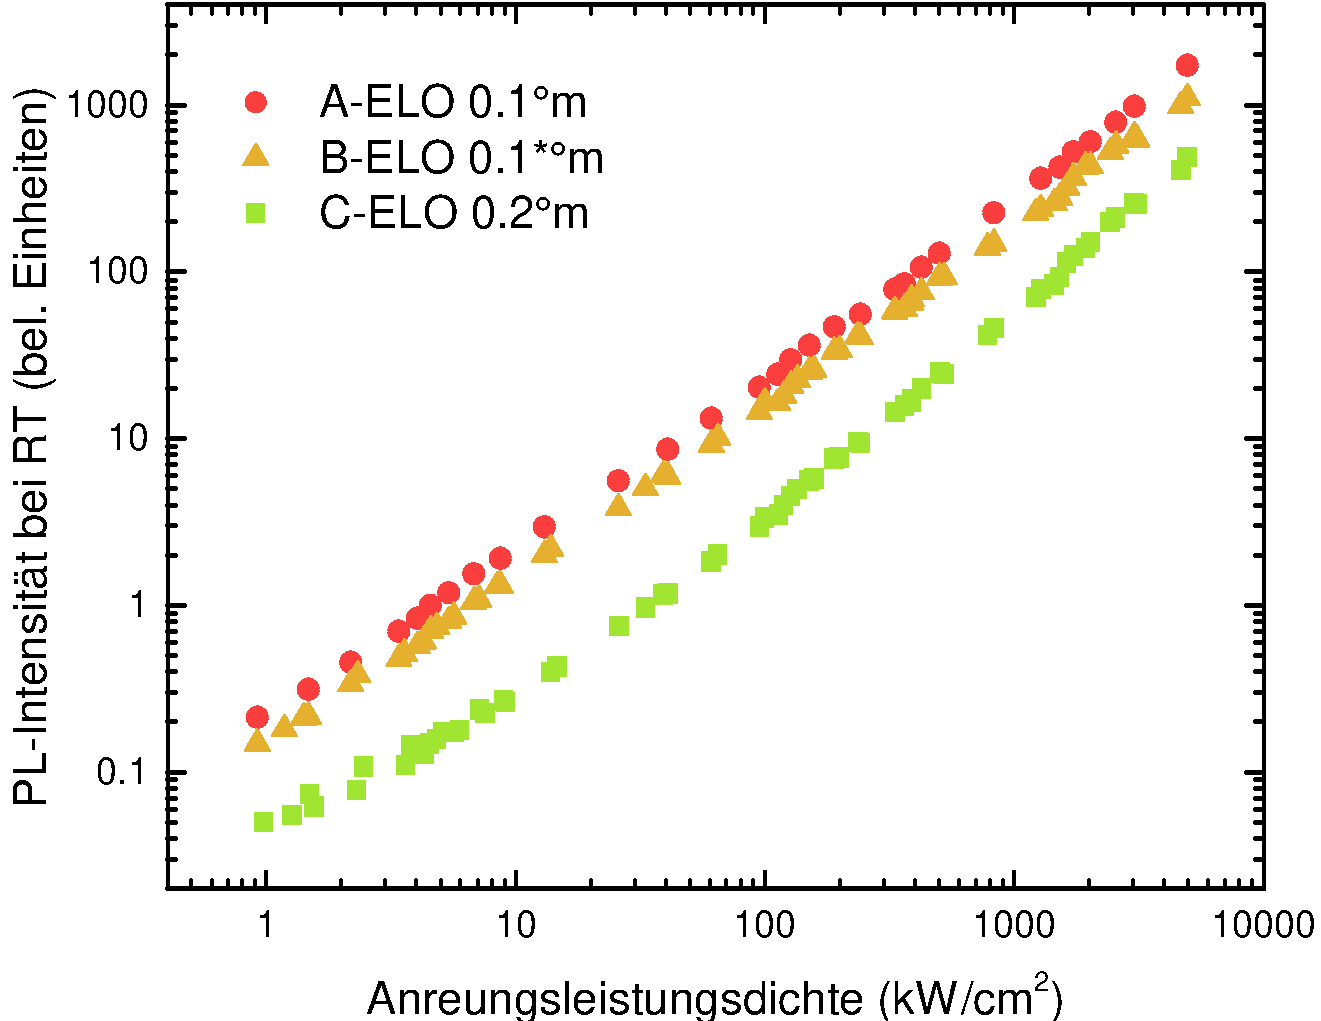
\includegraphics[width=\textwidth]{Bilder/TS4045/intRT.pdf}
    \label{}
  \end{minipage}
	\hfill
  \begin{minipage}[t]{0.49\textwidth}
    \centering
    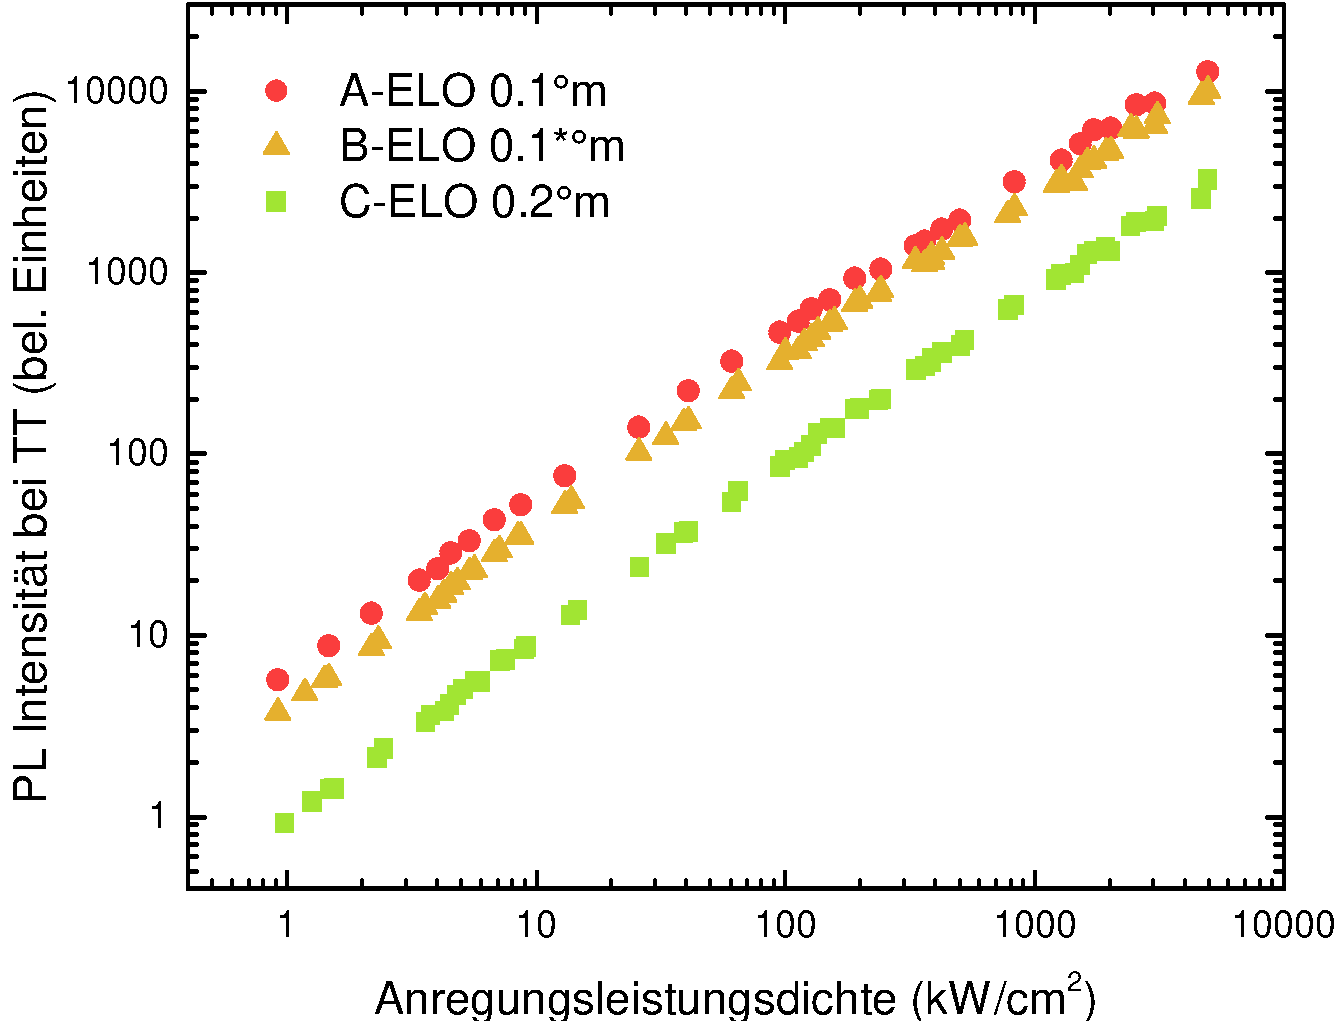
\includegraphics[width=\linewidth]{Bilder/TS4045/intTT.pdf}
    \label{}
  \end{minipage}
	\caption{Die integrierte Intensität in Abhängigkeit der Anregungsleistungsdichte bei Raum- und Tieftemperatur. }
\end{figure}
%